

\chapter{Introduction}
\label{chapter:introduction}

This chapter provides an introduction to the topic of the dissertation. It describes the problems that were tried to be solved and the motivation behind them.
\section{Motivation}
Cultural and archaeological heritage is one of the most important vehicles of cultural diversity and a way of preserving our history so that we can learn from the past and improve the future. Archaeology provides tools to understand how societies functioned and why the world and human society have changed.

Discovering a site rich in historical artifacts is every archaeologist's dream. Revealing to humanity a piece of its history that has been hidden for centuries or millennia is an arduous task that can result from successive trials and errors. To mitigate the costs associated with this activity, investments are being made in the development of artificial intelligence technologies\cite{bravenewworld} capable of indicating, with significant accuracy geographical regions where archaeological objects are more likely to be found. In this way, the excavation team can work more efficiently, saving time and money.

One of the reasons for this dissertation is the fact that the most common collection of archaeological information consists of walks in large fields. The ODDYSEY project consists in automating this process, using methods that have been increasingly used in archaeology in recent years, such as artificial intelligence and \ac{lidar}, which is encouraged by UNESCO and scientific communities\cite{asmr}, including all remote sensing techniques.
Remote sensing is the name given to all non-invasive techniques that use non-direct contact to observe targets of interest, either on the surface of the earth or from below, one of which is \ac{lidar}.

\ac{lidar} is a technology that uses light lasers to measure the distance of objects, allowing the creation of 3D models of the environment. By measuring the time it takes for the light to travel to the object and back, \ac{lidar} can accurately determine the distance to the object.

Another technique that has been used extensively with remote sensing in recent years is artificial intelligence, specifically convolutional neural networks (CNN). This technique allows the algorithm itself to learn through training the necessary filters to extract relevant features from images, which can be automatically adapted to different types of data and contexts. In addition, convolutional neural networks are capable of handling high-resolution and complex images, enabling higher accuracy in real-time object detection and classification. This makes remote sensing even more effective.


The utilization of artificial intelligence tools has experienced a rapid surge in recent years\cite{aumentoexpDL}. Various techniques, such as classical random forest machine learning, have been employed to identify archaeological mounds in regions like Mesopotamia, Pakistan, and Jordan \cite{LIDARCOMDL}. The adoption of deep learning techniques has seen a notable increase in conjunction with \ac{lidar} technology, likely due to the prevalence of tubular structures with archaeological significance worldwide \cite{LIDARCOMDL}. Among the subjects investigated in this dissertation are tumuli, which are also characterized by their tubular and uniform nature.


\section{Objectives}
The objective of the ODYSSEY project, funded by the COMPETE - Competitiveness and Internationalization Thematic Operational Program and the Regional Operational Programs, in its FEDER component, within the PORTUGAL2020 program, is to develop an integrated geographic information platform for archaeologists and heritage technicians, which allows the consolidation of different sources of heritage information, whether public or private, or directly from the field for specific purposes, using non-intrusive methods (e. g, LiDAR, multispectral imaging) and automate their further processing to identify archaeological elements and produce complementary information.

The project is divided into two parts, the pre-processing of LiDAR data and the detection of archaeological sites. In this dissertation only the detection part was done, having already access to the processed data, in the form of 4 \ac{lrm} images, each representing a sub-area of Alto Minho.


\begin{figure}[H]
\centering
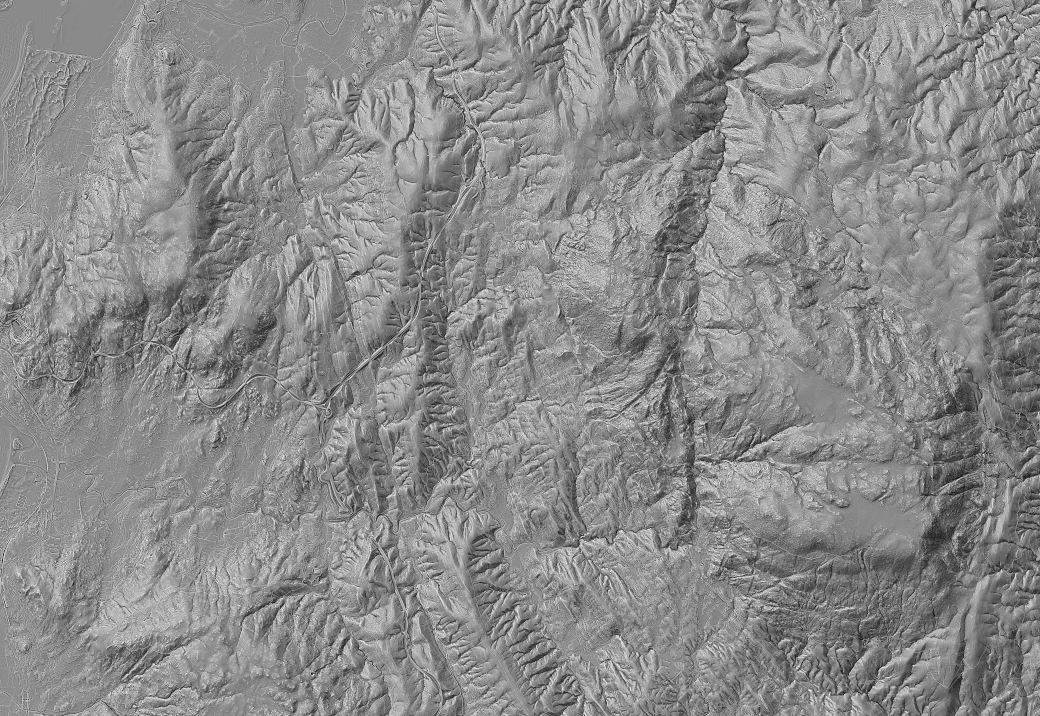
\includegraphics[height=6cm]{images/exampleLRM.png}
\caption{Example of a region from the LRM image of Viana do Castelo}

\end{figure}


To achieve this goal, the 4 LRM images were processed to create a dataset to train the two chosen deep learning models, \ac{yolo} and Unet, and augmentation techniques were applied. Finally, a Local Outlier Factor (LOF) model was trained on the LiDAR data to validate the results.

Finally, full inference was performed on all 4 \ac{lrm} images in an attempt to find undiscovered archaeological sites.

\section{Dissertation Structure}
The dissertation is divided into 6 chapters. In the first chapter an introduction is given to the topic and the motivation behind it. In the second chapter, the method of obtaining archelogical data is discussed. In the third chapter, it is explained how the datasets were created. Chapter 4 is about YOLOv7 and how it was used. Chapter 5 is about Unet and segmentation and finally chapter 6 is a conclusion.
